%%%%%%%%%%%%%%%%%%%%%%%%%%%%%%%%%%%%%%%%%%%%%%%%%%%%%%%%%%%%%%%%%%%%%%%%%%%%%%%
% CAPÍTULO 1 – INTRODUÇÃO
%%%%%%%%%%%%%%%%%%%%%%%%%%%%%%%%%%%%%%%%%%%%%%%%%%%%%%%%%%%%%%%%%%%%%%%%%%%%%%%

\chapter{Introdução}
\label{sec:introducao}

A digitalização dos serviços públicos surge como uma resposta eficaz à necessidade de modernização dos processos judiciais, conforme destacado em diversos estudos. O Sistema Eletrônico de Execução Unificado (SEEU) destaca-se como uma ferramenta essencial para a centralização e gestão dos processos no âmbito da execução penal, devido à crescente demanda por maior agilidade e precisão na recuperação de informações \cite{divald2021e-estonia}.

A relevância deste tema é evidenciada pela busca de superação dos desafios associados à consulta manual em um vasto acervo documental, um processo que se revela moroso, sujeito a inconsistências e, por conseguinte, propenso a retardar a tomada de decisão. O estudo "e-Estonia: A digital society for the transition to formality" ilustra como a digitalização pode promover maior transparência e eficiência, uma vez que "tudo no mundo online deixa uma rastreabilidade" \cite{divald2021e-estonia}.

No contexto atual, tecnologias que combinam Inteligência Artificial (IA) e modelos de linguagem de grande porte, em especial as técnicas de Retrieval-Augmented Generation (RAG), apresentam-se como soluções inovadoras. Essas técnicas permitem a integração de bases de dados externas com a geração de respostas contextualizadas, otimizando a recuperação de informações e possibilitando consultas em linguagem natural que fornecem resultados baseados em documentos originais de maneira rápida e precisa.

Este trabalho tem como objetivo desenvolver uma pipeline de RAG para processamento e disponibilização dos dados públicos do SEEU, principalmente os dados de suporte. Através de uma interface de chatbot, os operadores do Direito terão a capacidade de realizar buscas de forma intuitiva, obtendo respostas consistentes e contextualizadas. Além disso, a implementação de uma API para acesso externo amplia as possibilidades de integração com outros sistemas e serviços, contribuindo para a modernização do sistema Judiciário e para a transformação digital na execução penal.

%%%%%%%%%%%%%%%%%%%%%%%%%%%%%%%%%%%%%%%%%%%%%%%%%%%%%%%%%%%%%%%%%%%%%%%%%%%%%%%
% Seção 1.1 – Objetivos
%%%%%%%%%%%%%%%%%%%%%%%%%%%%%%%%%%%%%%%%%%%%%%%%%%%%%%%%%%%%%%%%%%%%%%%%%%%%%%%

\section{Objetivos}
\label{sec:objetivos}

\subsection{Objetivo Geral}
Desenvolver uma pipeline de Retrieval-Augmented Generation (RAG) para otimizar a recuperação e disponibilização de dados públicos no Sistema Eletrônico de Execução Unificado (SEEU), visando a modernização dos processos judiciais na esfera da execução penal e a promoção de uma gestão mais eficiente e transparente por meio da integração de tecnologias de Inteligência Artificial e interfaces de usuário intuitivas, como um chatbot, além de possibilitar a integração com outros sistemas através de uma API para acesso externo.

\subsection{Objetivos Específicos}
\begin{enumerate}[label=\arabic*.]
  \item Coletar e organizar os dados públicos do SEEU, principalmente os documentos de suporte;
  \item Realizar a vetorização desses dados em um banco de dados vetorial (Elasticsearch, OpenSearch ou PostgreSQL+pgvector);
  \item Desenvolver uma pipeline que conecte o índice vetorial ao LLM selecionado, criando mecanismos para consultas precisas;
  \item Realizar testes de integração para avaliar a eficiência e a qualidade das respostas geradas;
  \item Criar uma interface de chatbot integrada à pipeline de RAG e ao LLM para interação em tempo real;
  \item Conduzir testes de usabilidade e implementar ajustes para aprimorar a experiência do usuário;
  \item Implementar uma API REST documentada para consumo externo;
  \item Preparar o ambiente para deployment, considerando aspectos de segurança e escalabilidade.
\end{enumerate}

%%%%%%%%%%%%%%%%%%%%%%%%%%%%%%%%%%%%%%%%%%%%%%%%%%%%%%%%%%%%%%%%%%%%%%%%%%%%%%%
% Seção 1.2 – Trabalhos Correlatos
%%%%%%%%%%%%%%%%%%%%%%%%%%%%%%%%%%%%%%%%%%%%%%%%%%%%%%%%%%%%%%%%%%%%%%%%%%%%%%%

\section{Trabalhos Correlatos}
\label{sec:trabalhos-correlatos}

\textbf{Edwards (2024)} propõe uma abordagem híbrida que combina RAG com grafos de conhecimento para relatórios de acreditação em educação superior. Embora semelhante na tecnologia RAG, difere no domínio de aplicação (educação vs. execução penal), exigindo adaptações metodológicas para atender às necessidades do SEEU.

\textbf{Aquino (2024)} investiga extração de informações de documentos jurídicos brasileiros com RAG, apontando estratégias para mitigar alucinações e validar experimentalmente resultados. Tais estratégias são fundamentais para aumentar a confiabilidade do sistema proposto.

\textbf{Pujiono et al. (2024)} desenvolvem um chatbot RAG para consultas em agências públicas, empregando métricas de similaridade (\emph{cosine similarity}) para avaliar relevância das respostas. Este trabalho expande essa aplicação ao domínio penal e adiciona interoperabilidade via API.

%%%%%%%%%%%%%%%%%%%%%%%%%%%%%%%%%%%%%%%%%%%%%%%%%%%%%%%%%%%%%%%%%%%%%%%%%%%%%%%
% Seção 1.3 – Solução Proposta
%%%%%%%%%%%%%%%%%%%%%%%%%%%%%%%%%%%%%%%%%%%%%%%%%%%%%%%%%%%%%%%%%%%%%%%%%%%%%%%

\section{Solução Proposta}
\label{sub:solucao-proposta}

A solução consiste em uma pipeline de RAG com as etapas:
\begin{itemize}[label=\textbullet]
  \item Coleta automatizada de documentos oficiais do SEEU;
  \item Pré-processamento (limpeza, segmentação em 
  \emph{chunks});
  \item Vetorização por embeddings e indexação em banco vetorial;
  \item Orquestração via LangChain entre FAISS/OpenSearch e LLM;
  \item Exposição do serviço por chatbot e API REST.
\end{itemize}

Essa arquitetura visa modernizar a consulta ao SEEU, reduzir tempo de busca e alucinações, e integrar-se a iniciativas do CNJ, PNUD e ONU.

%%%%%%%%%%%%%%%%%%%%%%%%%%%%%%%%%%%%%%%%%%%%%%%%%%%%%%%%%%%%%%%%%%%%%%%%%%%%%%%
% CAPÍTULO 2 – FUNDAMENTAÇÃO TEÓRICA E REVISÃO DE LITERATURA
%%%%%%%%%%%%%%%%%%%%%%%%%%%%%%%%%%%%%%%%%%%%%%%%%%%%%%%%%%%%%%%%%%%%%%%%%%%%%%%

\chapter{Fundamentação Teórica e Revisão de Literatura}
\label{chap:fundamentacao_literatura}

\section{Bancos de Dados Vetoriais}
Bancos de dados vetoriais são sistemas especializados para armazenar, indexar e consultar embeddings gerados por modelos de aprendizado de máquina, permitindo buscas semânticas de alta dimensionalidade \cite{taipalus2024vector}. Esses sistemas habilitam aplicações como:
\begin{itemize}[label=\textbullet]
  \item Sistemas de recomendação;
  \item Busca semântica;
  \item Reconhecimento de padrões;
  \item Integração com pipelines de IA.
\end{itemize}

\subsection{Comparativo de Soluções}
\begin{description}
  \item[Elasticsearch/OpenSearch:] escalável e distribuído, suporta vetorização via plugins. Menos maduro para consultas de alta dimensionalidade.
  \item[PostgreSQL + pgvector:] integra dados relacionais e vetoriais; desempenho inferior em escala massiva.
  \item[Milvus:] especializado e altamente otimizado, porém requer manutenção especializada.
  \item[FAISS:] biblioteca eficiente de ANNS; necessita de sistema auxiliar para funcionalidades completas.
  \item[Weaviate:] banco vetorial com recursos de grafo; exige configuração avançada.
  \item[Oracle/IBM Vector DB:] soluções corporativas integradas a seus respectivos ecossistemas; custo e flexibilidade variáveis.
\end{description}

\section{Large Language Models}
Modelos Transformer (GPT, BERT, LLama) passam por \emph{pre-training} em grandes corpora e \emph{fine-tuning} em domínios jurídicos para evitar alucinações e capturar nuances do linguajar penal \cite{vaswani2017attention,naveeda2024comprehensive}.

\section{Retrieval-Augmented Generation}
O RAG integra dois módulos:
\begin{enumerate}[label=\arabic*.]
  \item \textbf{Retriever:} converte consultas e documentos em embeddings e recupera trechos relevantes;
  \item \textbf{Generator:} utiliza LLM para formular respostas fundamentadas.
\end{enumerate}

Variantes:
\begin{itemize}[label=\textbullet]
  \item \emph{RAG-Sequence}: margina sobre documentos completos;
  \item \emph{RAG-Token}: escolhe fonte para cada token.
\end{itemize}

Desafios incluem latência, atualização em tempo real e coerência textual \cite{saleافغان미}.

%%%%%%%%%%%%%%%%%%%%%%%%%%%%%%%%%%%%%%%%%%%%%%%%%%%%%%%%%%%%%%%%%%%%%%%%%%%%%%%
% CAPÍTULO 3 – TECNOLOGIAS (revisado)
%%%%%%%%%%%%%%%%%%%%%%%%%%%%%%%%%%%%%%%%%%%%%%%%%%%%%%%%%%%%%%%%%%%%%%%%%%%%%%%

\chapter{Tecnologias}
\label{chap:tecnologias}

\section{Linguagem e Bibliotecas Principais}
\begin{itemize}[label=\textbullet]
  \item \textbf{Python} – linguagem base, com extensas bibliotecas para NLP e ML (\cite{python2024});
  \item \textbf{Pandas} – manipulação de dados tabulares e pré-processamento de textos (\cite{pandas2024});
  \item \textbf{NumPy} – operações vetoriais e matrizes de alto desempenho.
\end{itemize}

\section{Indexação e Recuperação Vetorial}
\subsection{OpenSearch}
Mecanismo de busca distribuída com suporte nativo a buscas vetoriais via plugins; ótimo para cenários de alta disponibilidade e grandes volumes de dados (\cite{taipalus2024vector}).

\subsection{FAISS}
Biblioteca de similaridade aproximada desenvolvida pelo Facebook, altamente otimizada para bilhões de vetores, mas depende de um sistema auxiliar para metadados e persistência (\cite{facebookresearch2024faiss}).

\subsection{Milvus e Weaviate}
Soluções especializadas de código-aberto com integração a grafos (Weaviate) e suporte a esquemas de indexação avançados (Milvus). Indicadas para aplicações críticas de IA.

\section{Modelos de Linguagem}
\subsection{LLama}
Modelo open-source eficiente, customizável para domínios específicos, incluindo jurídico.

\subsection{Hugging Face Transformers}
Framework que fornece acesso a dezenas de modelos pré-treinados, tokenizadores e utilitários de pipeline (\cite{huggingface2024transformers}).

\section{Orquestração de Pipeline}
\subsection{LangChain}
Framework modular que conecta retriever (FAISS/OpenSearch) e generator (LLM), permitindo composição de fluxos e gerenciamento de prompts (\cite{langchain2024}).

\subsection{Controle de Prompt e Fallback}
Implementação de lógica para reformulação de prompts e fallback a dados oficiais caso o LLM retorne resposta vaga.

\section{Infraestrutura e Deployment}
\subsection{Docker e Kubernetes}
Containerização para padronização de ambientes e orquestração em cluster, garantindo escalabilidade horizontal e isolamento.

\subsection{API REST com Flask}
Microframework escolhido pela maturidade e simplicidade, expondo endpoints para chatbot e integração externa (\cite{flask2024}).

%%%%%%%%%%%%%%%%%%%%%%%%%%%%%%%%%%%%%%%%%%%%%%%%%%%%%%%%%%%%%%%%%%%%%%%%%%%%%%%
% CAPÍTULO 4 – METODOLOGIA (revisado)
%%%%%%%%%%%%%%%%%%%%%%%%%%%%%%%%%%%%%%%%%%%%%%%%%%%%%%%%%%%%%%%%%%%%%%%%%%%%%%%

\chapter{Metodologia}
\label{chap:metodologia}

\section{Arquitetura da Pipeline}
A pipeline combina quatro estágios principais: ingestão, pré‐processamento, indexação e geração. Cada estágio é containerizado e orquestrado via Kubernetes (Figura~\ref{fig:arquitetura_pipeline}).

\section{Coleta de Dados}
\begin{itemize}[label=\textbullet]
  \item Raspagem automática dos portais do CNJ usando Python e bibliotecas como \texttt{requests} e \texttt{BeautifulSoup};
  \item Agendamento via \emph{cron} ou Airflow para verificações diárias de novos documentos.
\end{itemize}

\section{Pré-processamento e Segmentação}
\begin{enumerate}[label=\\arabic*.]
  \item Conversão PDF→texto com \texttt{pdfplumber};
  \item Remoção de cabeçalhos, rodapés e caracteres especiais;
  \item Divisão em \emph{chunks} de 500–1\,000 tokens para otimizar a busca local.
\end{enumerate}

\section{Engenharia de Embeddings}
Escolha de modelo de embedding (BERTimbau ou OpenAI), parametrização de tamanho e normalização para garantir coerência semântica.

\section{Indexação e Armazenamento}
\begin{itemize}[label=\textbullet]
  \item Indexação dos embeddings em OpenSearch/FAISS com metadados (origem, data, posição);
  \item Definição de métricas de similaridade (cosine similarity) e thresholds de corte.
\end{itemize}

\section{Orquestração e Consulta}
Implementação em LangChain:
\begin{itemize}[label=\textbullet]
  \item Conversão da consulta em embedding;
  \item Recuperação dos top-k \emph{chunks};
  \item Geração da resposta pelo LLM, mesclando múltiplas fontes se necessário (\emph{RAG-Token}).
\end{itemize}

\section{Desenvolvimento do Chatbot e da API}
\begin{itemize}[label=\textbullet]
  \item Chatbot baseado em WebSocket para interação síncrona;
  \item Endpoints RESTful em Flask para consultas e feedback de usabilidade.
\end{itemize}

\section{Avaliação e Métricas}
\begin{itemize}[label=\textbullet]
  \item Precisão, recall e F1-Score em um conjunto de questões de benchmark (fase de testes);
  \item Ensaios de usabilidade qualitativos com operadores do Direito para avaliar intuitividade e confiança.
\end{itemize}

\section{MLOps e Monitoramento}
\begin{itemize}[label=\textbullet]
  \item Pipelines de CI/CD para build e deploy automáticos;
  \item Monitoramento de latência e acurácia em produção, com alertas para queda de desempenho;
  \item Feedback loop para re-treinamento periódico com dados reais de uso.
\end{itemize}

\begin{figure}[h!]
  \centering
  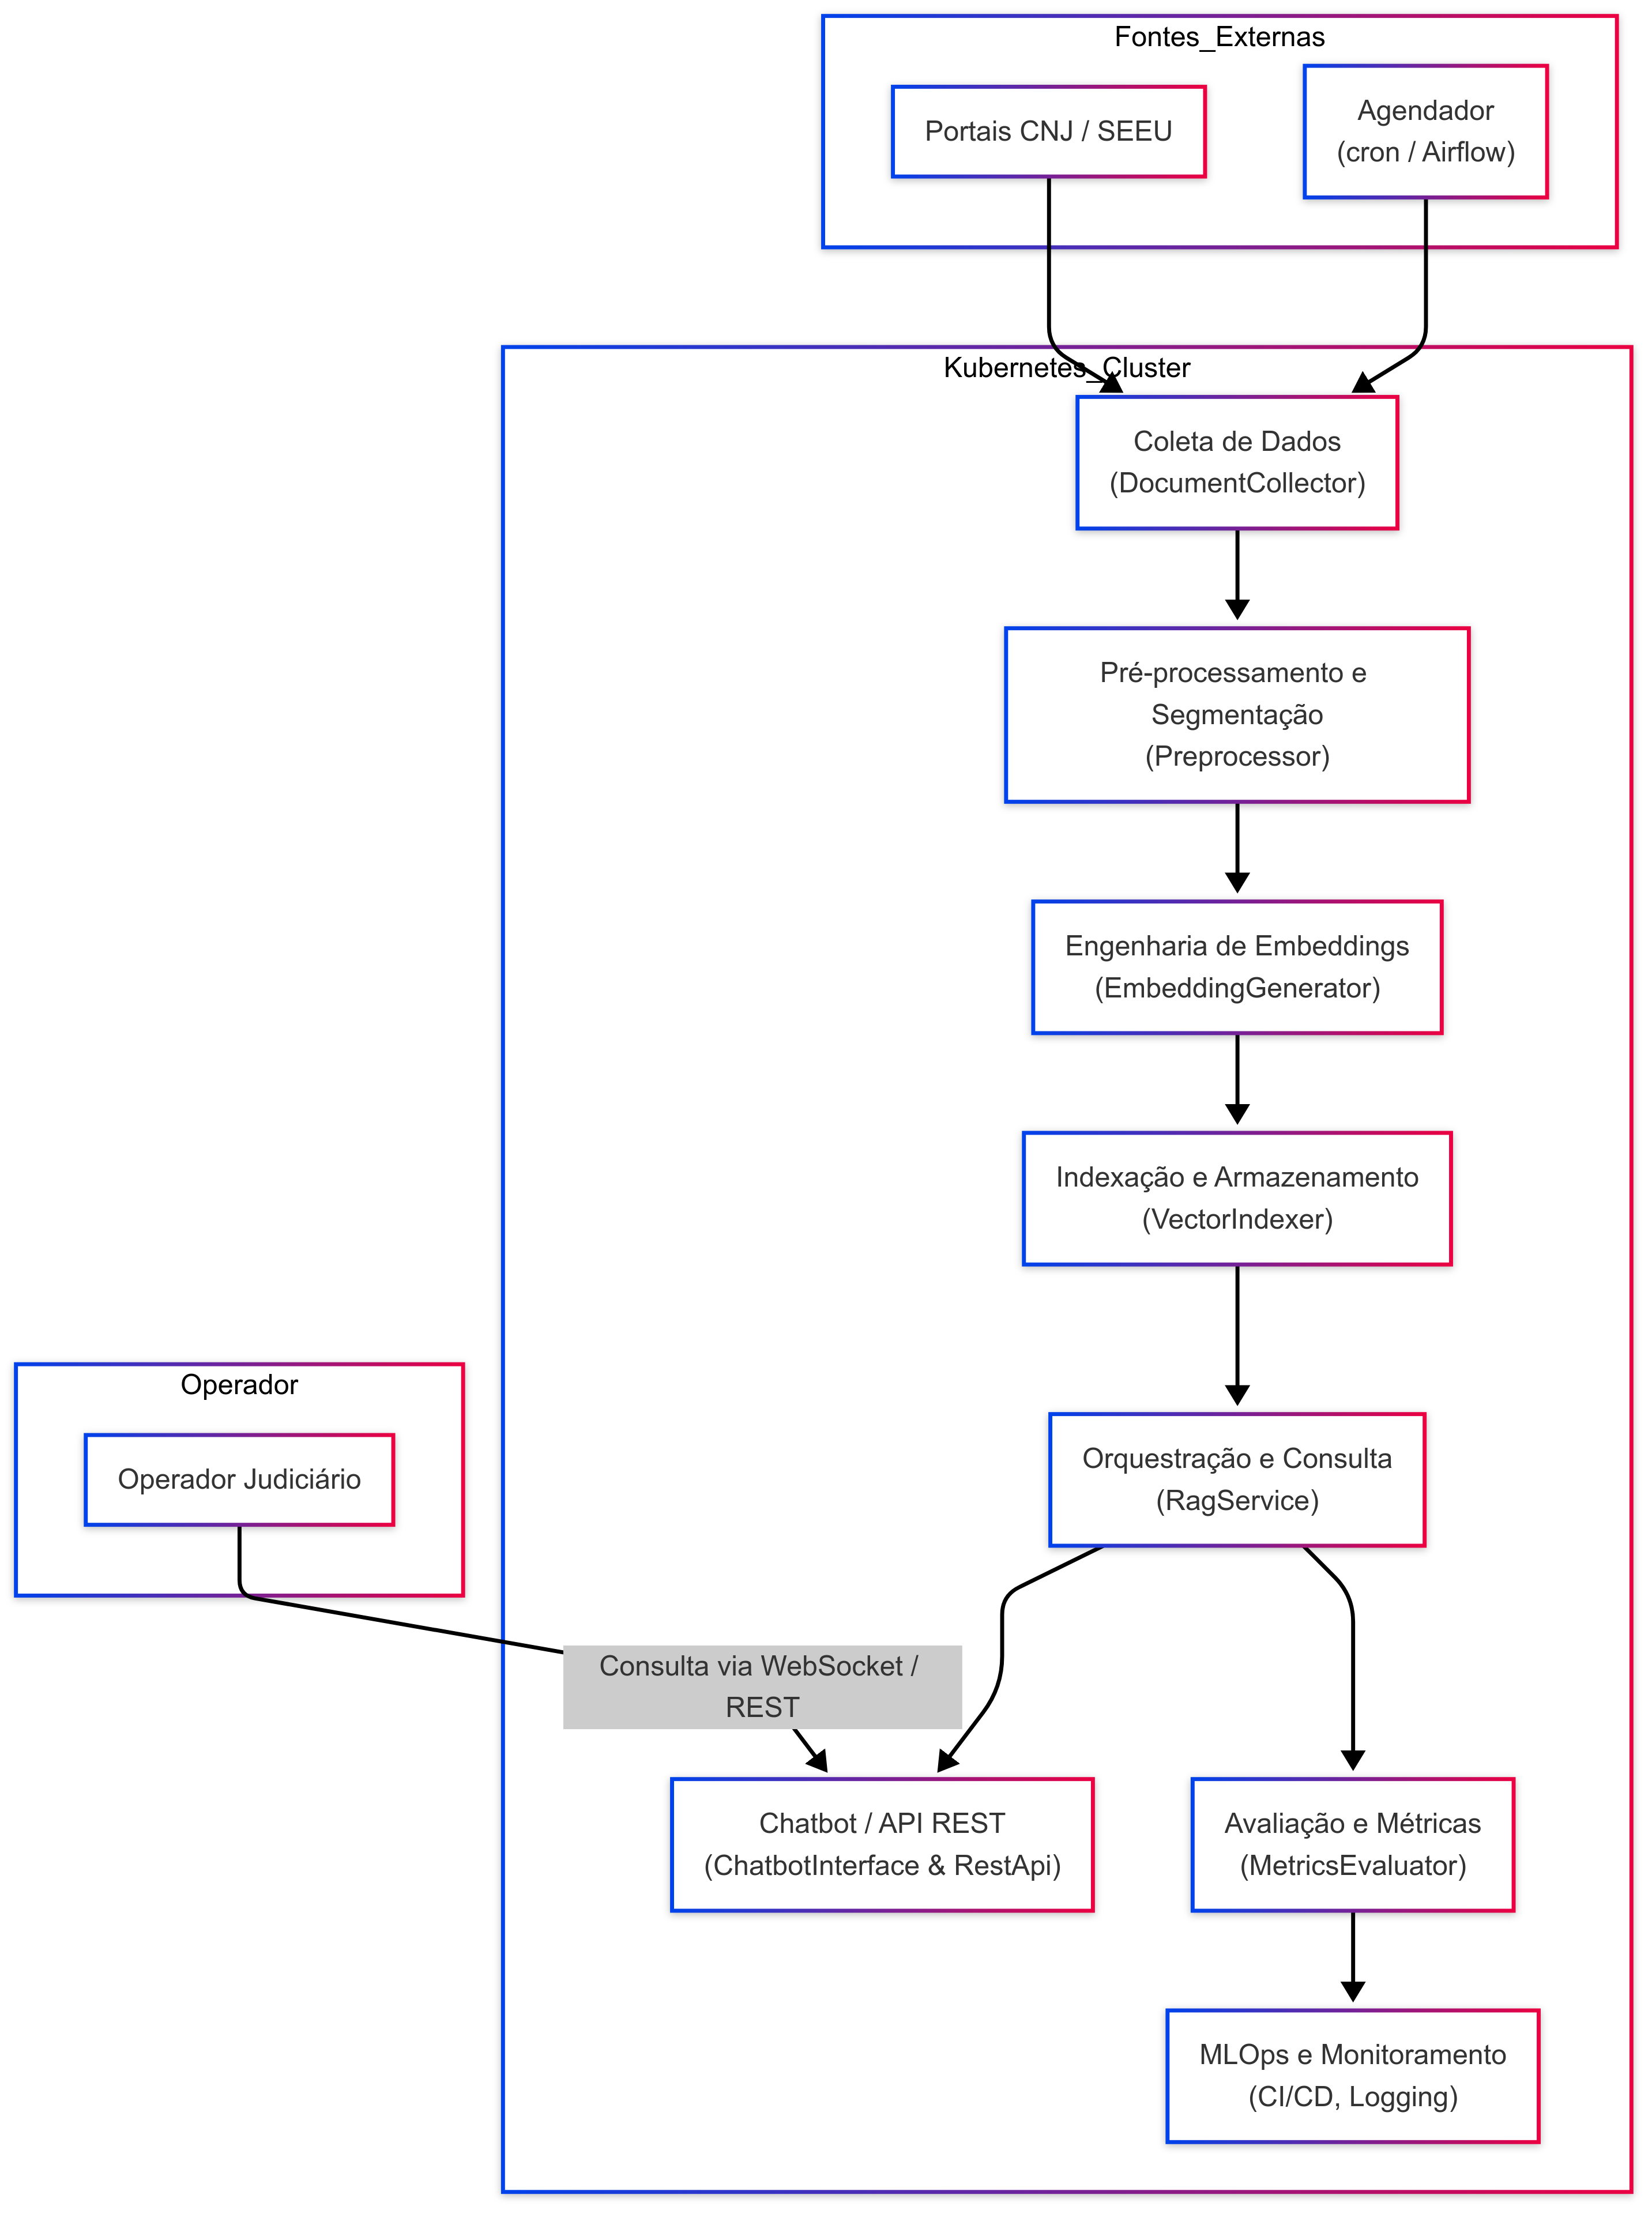
\includegraphics[width=0.8\textwidth]{04-figuras/arquitetura_pipeline.png}
  \caption{Arquitetura geral da pipeline RAG.}
  \label{fig:arquitetura_pipeline}
\end{figure}


%%%%%%%%%%%%%%%%%%%%%%%%%%%%%%%%%%%%%%%%%%%%%%%%%%%%%%%%%%%%%%%%%%%%%%%%%%%%%%%
% CAPÍTULO 5 – RESULTADOS ESPERADOS
%%%%%%%%%%%%%%%%%%%%%%%%%%%%%%%%%%%%%%%%%%%%%%%%%%%%%%%%%%%%%%%%%%%%%%%%%%%%%%%

\chapter{Resultados Esperados}
\label{chap:resultados}

\begin{itemize}[label=\textbullet]
  \item Redução de ≥80\% no tempo de busca;
  \item Precisão ≥0,85, recall ≥0,80, F1-Score ≥0,82;
  \item Alucinações ≤5\%;
  \item Latência média <1 s;
  \item Escalabilidade via Docker/Kubernetes.
\end{itemize}

%%%%%%%%%%%%%%%%%%%%%%%%%%%%%%%%%%%%%%%%%%%%%%%%%%%%%%%%%%%%%%%%%%%%%%%%%%%%%%%
% CAPÍTULO 6 – CONCLUSÕES
%%%%%%%%%%%%%%%%%%%%%%%%%%%%%%%%%%%%%%%%%%%%%%%%%%%%%%%%%%%%%%%%%%%%%%%%%%%%%%%

\chapter{Conclusões}
\label{chap:conclusoes}

A pipeline proposta demonstra a viabilidade de aplicar RAG ao SEEU, alinhando-se a iniciativas de Justiça 4.0 e ODS 16. Com redução de tempo e maior precisão, espera-se uma execução penal mais transparente e eficiente. Trabalhos futuros podem expandir o escopo para outros domínios jurídicos e refinar embeddings em português jurídico.